\chapter{Introduction}
Les recherches sur la physique fondamentale requièrent des installations hors normes, défiant les limites de ce que l'on considère comme possible. Les installations du CERN, laboratoire européen situé en Suisse qui pratique des expériences à la fine pointe de la technologie est un laboratoire dont le financement est de nature publique et dont la connaissance est diffusée. Une représentation de l'ensemble de l'installation est présentée à la figure \ref{CERN} Ce laboratoire utilise des techniques existantes, mais repousse les limites de précision et de fiabilité. Le sujet d'étude de ce projet de fin d'études porte sur une alimentation électronique visant à remplacer une alimentation existante. Le remplacement doit permettre une augmentation substantielle de l'énergie des faisceaux de protons. Le rôle de l'équipe Électrosim consiste à reproduire l'alimentation en développement au CERN sur  trois simulateurs: SimPowerSystems (SPS), PSIM ainsi que sur un simulateur temps réel, fourni par la compagnie Opal-RT. Le client direct du projet est le laboratoire LEEPCI, de l'Université Laval, qui désire d'une part, étudier la méthode d'implantation de l'alimentation électronique du CERN en la reproduisant sur trois plateformes de simulation et d'autres part, valider l'implantation des modèles de simulations en comparant les résultats sur les différentes plateformes. Le projet vise à obtenir une compréhension théorique des choix techniques effectués par les ingénieurs du CERN en étudiant les résultats de simulation. Le rapport de détaille en plusieurs sections: soit une explication détaillée du contexte et de la problématique entourant l'alimentation électronique, une énumération des besoins et des objectifs rattachés au projet, une présentation du cahier des charges sous le format d'un diagramme des propriétés fonctionnelles,   l'explication de la méthodologie employée, une analyse simplifiée des sous-systèmes implantés et une analyse détaillée du système intégré

\begin{figure}[htb]
\centering
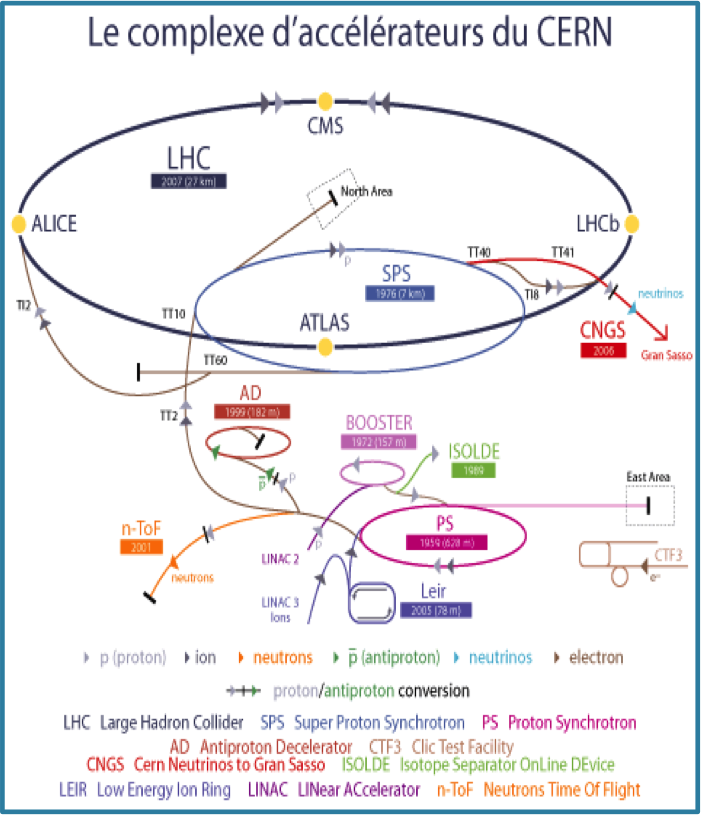
\includegraphics[scale=0.8]{fig/CERN.png}
\caption{Représentation schématique de l'implantation du complexe d'accélérateurs du CERN}
\label{CERN}
\end{figure}
